\documentclass[11pt,a4paper]{article}

\usepackage[utf8]{inputenc}
\usepackage[T1]{fontenc}
\usepackage{amsmath,amssymb,amsfonts}
\usepackage{geometry}
\usepackage{graphicx}
\usepackage{hyperref}
\usepackage{booktabs}
\usepackage{float}
\usepackage{xcolor}

\geometry{
    a4paper,
    total={170mm,257mm},
    left=20mm,
    top=20mm,
}

\hypersetup{
    colorlinks=true,
    linkcolor=blue,
    filecolor=magenta,
    urlcolor=cyan,
}

\title{\vspace{-2cm}Knowledge Manifold:\\Mathematical Overview}
\date{}
\author{}

\begin{document}

\maketitle
\vspace{-1.5cm}

\tableofcontents
\vspace{0.5cm}

\section{Notation}

\begin{table}[H]
\centering
\begin{tabular}{ll}
\toprule
\textbf{Symbol} & \textbf{Definition} \\
\midrule
$N$ & Number of particles (teams) \\
$K$ & Number of preference dimensions ($K=3$, where dims 0,1 are skills) \\
$G$ & Grid resolution for the knowledge field ($G \times G$ cells) \\
$p_i \in [-1, 1]^K$ & Preference (skill) vector of particle $i$ \\
$F(p)$ & Hidden fitness landscape (the ceiling), $F \in [0, 1]$ \\
$M(c)$ & Knowledge manifold height at grid cell $c$, $M \in [0, 1]$ \\
$\text{cell}(p)$ & Grid cell containing preference vector $p$ \\
$w$ & Knowledge write rate (deposit amount per step) \\
$\sigma_{\text{diff}}$ & Gaussian diffusion standard deviation (in cells) \\
$\gamma$ & Exponential decay factor per step \\
$s_{\text{max}}$ & Maximum allowed slope (structural support constraint) \\
$\alpha$ & Exponential reward scale \\
$\beta$ & Reward growth bonus multiplier \\
$\sigma_i$ & Adaptive exploration noise level for particle $i$ \\
$v_{\text{frac}}$ & Fraction of particles designated as visionaries \\
$v_{\text{nudge}}$ & Visionary nudge rate toward the hidden global peak \\
\bottomrule
\end{tabular}
\end{table}

\section{Overview}

The base Social Dynamics Simulator models particles moving through a spatial domain $\mathbf{x}_i \in [0, L)^2$ and interacting via their preference vectors $\mathbf{p}_i \in [-1, 1]^K$. In the base model, social learning and movement are driven entirely by peer-to-peer interactions and spatial memory fields.

The \textbf{Knowledge Manifold} extension introduces a new environmental layer: an objective, shared surface representing the organization's accumulated discoveries over the preference (skill) space. Rather than preferences shifting solely based on peer popularity, particles now navigate a rugged landscape of objective utility.

Crucially, this introduces a two-layer architecture:
\begin{enumerate}
    \item \textbf{The Hidden Fitness Landscape $F$}: The objective truth of what combinations of skills are valuable. This acts as an absolute ceiling; knowledge cannot exceed reality.
    \item \textbf{The Knowledge Manifold $M$}: The \textit{known} utility surface. Particles perform noisy research to "push up" this manifold at their current preference coordinates.
\end{enumerate}

This creates a dynamic where teams must collaborate to build knowledge. Because of structural support constraints, a single team cannot build a tall, isolated spire of knowledge. Broad bases of shared understanding are required to support high peaks of specialized expertise. The resulting knowledge heights then feed back into the base social dynamics, causing talent to flow toward the most productive teams.

\section{The Hidden Fitness Landscape}

The hidden fitness landscape $F(p_0, p_1)$ defines the maximum possible knowledge at any point in the 2D skill space. It is constructed as a sum of Gaussian peaks representing distinct domains of knowledge, plus high-frequency spectral noise representing the ruggedness of real-world research.

\begin{equation}
F(p_0, p_1) = \sum_{j=1}^{N_{\text{peaks}}} h_j \exp\left(-\frac{\|p - c_j\|^2}{2s_j^2}\right) + \sum_{k=1}^{N_{\text{freqs}}} a_k \sin(2\pi f_k (p \cdot d_k) + \phi_k)
\end{equation}

The resulting landscape is normalized such that $F \in [0, 1]$.

\begin{figure}[H]
\centering
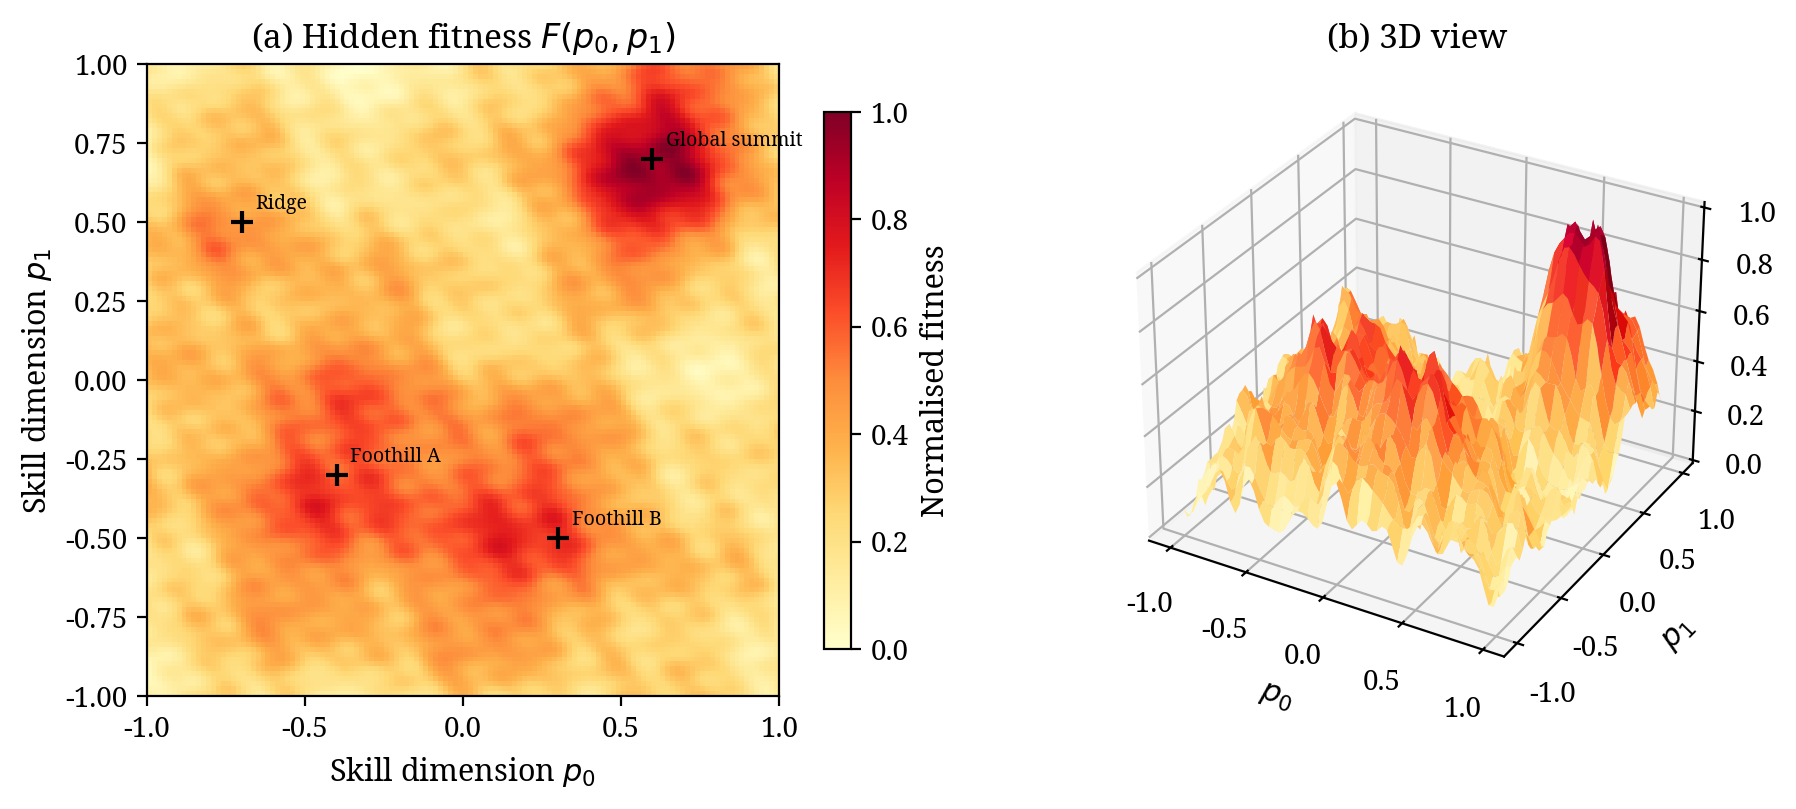
\includegraphics[width=0.9\textwidth]{figures/fig1_fitness_landscape.png}
\caption{The hidden fitness landscape $F(p_0, p_1)$. This acts as the absolute ceiling for the knowledge manifold. Regular particles cannot see this landscape; they only interact with the knowledge they have collectively built.}
\end{figure}

\section{Knowledge Field Dynamics}

The knowledge manifold $M$ is a $G \times G$ scalar grid. At each time step, particles attempt to deposit knowledge, subject to constraints, followed by diffusion and decay.

\subsection{Knowledge Deposit and the Fitness Ceiling}

Each particle $i$ attempts to add an amount $w$ (the write rate) to the manifold at its current cell $c = \text{cell}(p_i)$. The manifold is strictly bounded by the hidden fitness landscape:

\begin{equation}
M'(c) = \min(M(c) + w, F(c))
\end{equation}

\subsection{Structural Support Constraint}

Knowledge cannot be built in isolation. To prevent infinitely thin spires of knowledge, a structural support constraint enforces that no cell can be significantly higher than its local neighborhood. 

Let $\bar{M}_r(c)$ be the mean knowledge height in a neighborhood of radius $r$ around cell $c$. The height is constrained by a maximum slope parameter $s_{\text{max}}$:

\begin{equation}
M''(c) = \min(M'(c), \bar{M}_r(c) + s_{\text{max}})
\end{equation}

\textbf{Key insight:} This constraint means that a single team researching a narrow topic will quickly hit a ceiling. To build higher, multiple teams must research adjacent topics to raise the local mean, creating a broad base that supports a higher peak.

\begin{figure}[H]
\centering
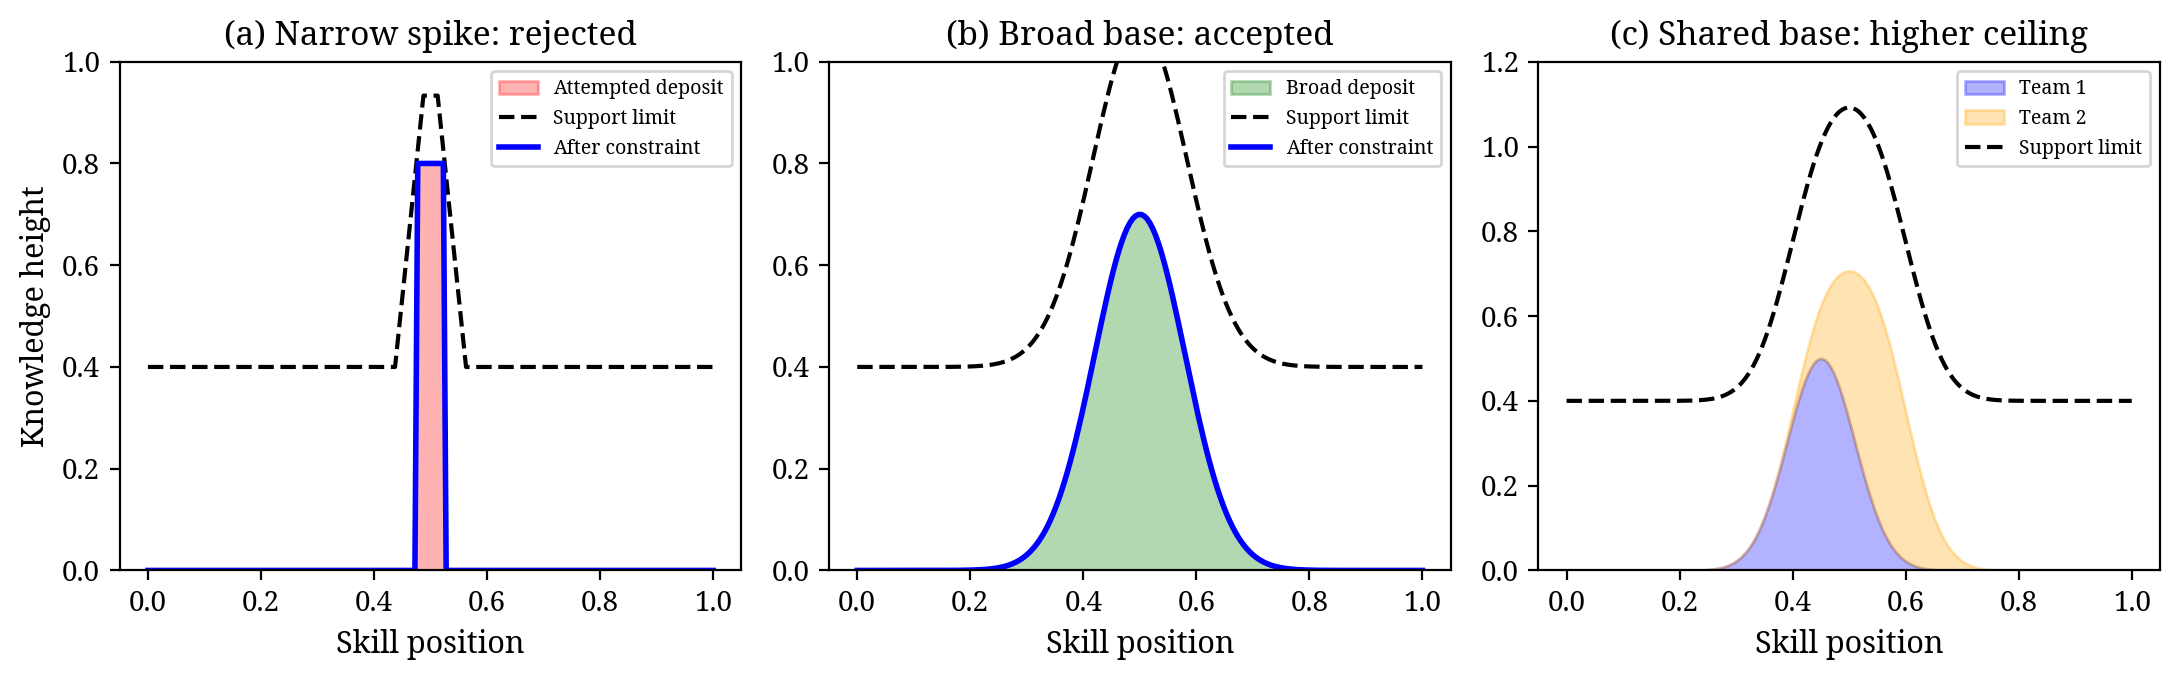
\includegraphics[width=\textwidth]{figures/fig2_structural_support.png}
\caption{Illustration of the structural support constraint. (a) A narrow deposit is rejected because it exceeds the support limit. (b) A broad deposit is accepted. (c) Two teams researching adjacent topics build a shared base, raising the support limit and allowing both to reach higher peaks.}
\end{figure}

\subsection{Diffusion and Decay}

The knowledge field diffuses spatially and decays over time, representing knowledge sharing and obsolescence:

\begin{equation}
M_{t+1} = \gamma \cdot (M'' * \mathcal{G}(\sigma_{\text{diff}}))
\end{equation}

where $*$ denotes convolution with a Gaussian kernel of standard deviation $\sigma_{\text{diff}}$, and $\gamma$ is the decay factor (typically very close to 1.0, e.g., 0.9999).

\begin{figure}[H]
\centering
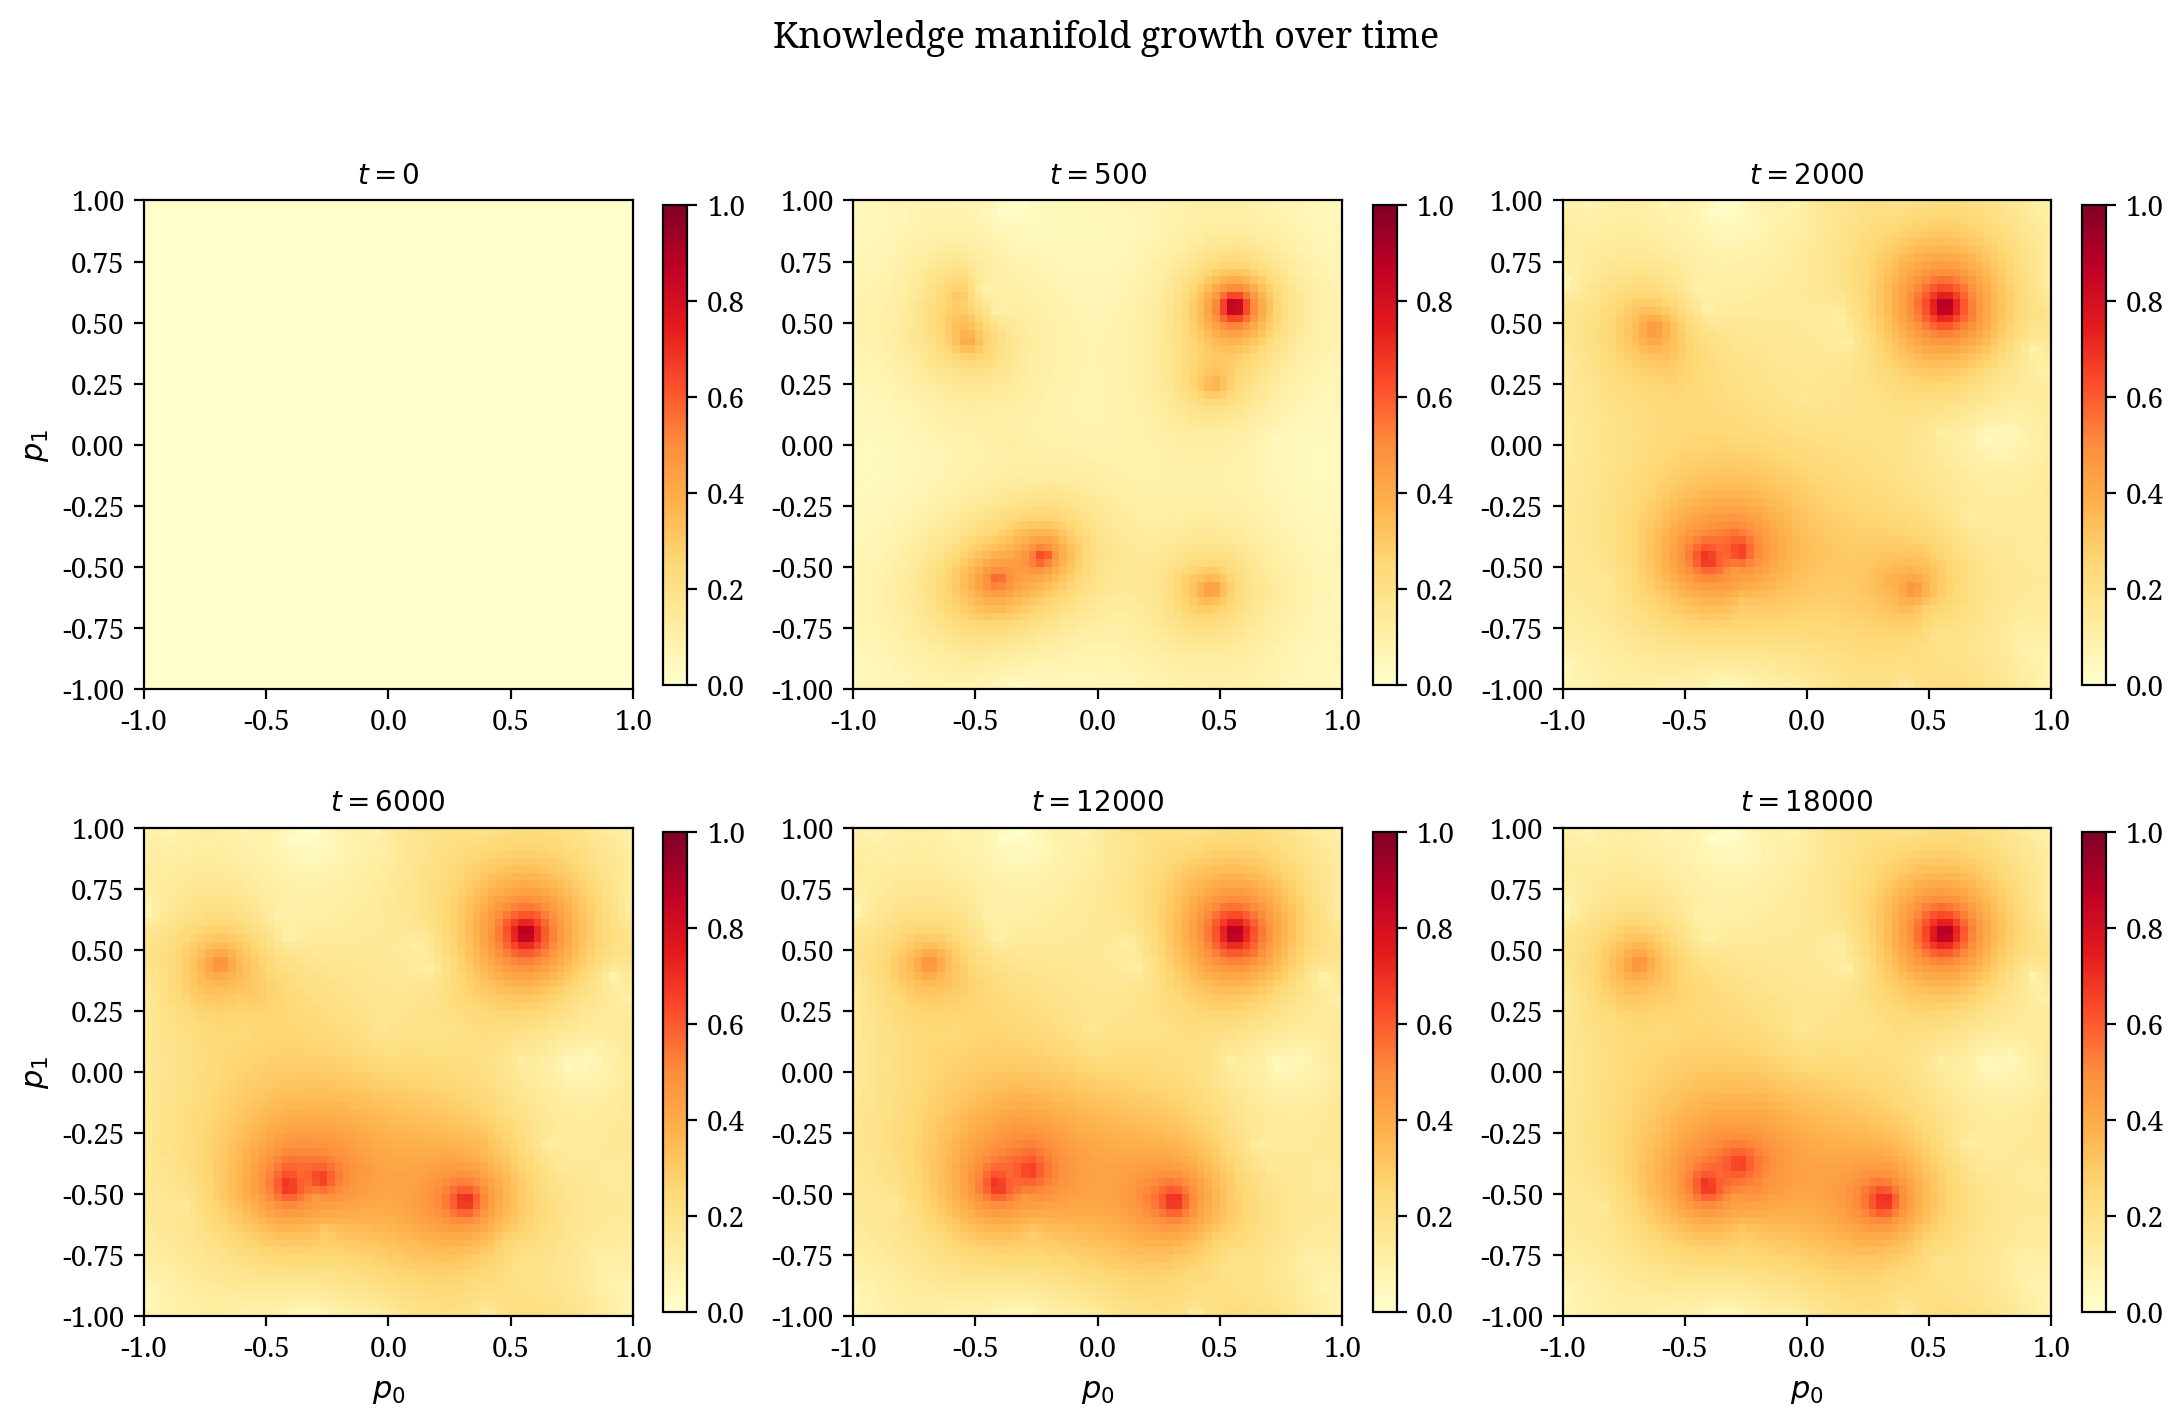
\includegraphics[width=\textwidth]{figures/fig4_knowledge_snapshots.png}
\caption{Time-lapse of the knowledge manifold growing from an initially flat state. Teams cluster around viable research areas, gradually building up the surface until it hits the hidden fitness ceiling.}
\end{figure}

\section{Particle Movement}

In the base model, particle preferences $\mathbf{p}_i$ shift primarily via the social learning rule (moving toward/away from neighbors) and the spatial memory field. 

The Knowledge Manifold introduces three additional forces to the skill dimensions ($p_0, p_1$) of the preference vector: knowledge gradient climbing, visionary nudges, and adaptive exploration noise. (The social dimension $p_2$ continues to be governed purely by the base social dynamics).

\subsection{Knowledge Gradient Climbing}

Regular particles have no access to the hidden fitness landscape. They can only climb the gradient of the \textit{known} manifold $M$:

\begin{equation}
v_{\text{climb}} = \eta_{\text{climb}} \frac{\nabla M(p)}{\|\nabla M(p)\|}
\end{equation}

This causes teams to drift toward established, known-good areas of research, creating a strong exploitative tendency.

\subsection{Visionary Nudge}

A small fraction of particles ($v_{\text{frac}}$, default 2\%) are designated as "visionaries". These rare individuals have an intuition for the hidden fitness landscape $F$ and receive a small nudge toward its local gradient:

\begin{equation}
v_{\text{vis}} = \eta_{\text{vis}} \frac{\nabla F(p)}{\|\nabla F(p)\|}
\end{equation}

This allows visionaries to lead the organization into entirely new, unexplored areas of the fitness landscape, overcoming the exploitative pull of the known manifold.

\subsection{Adaptive Exploration Noise}

To prevent particles from getting permanently stuck in local optima, they undergo random walks with an adaptive noise level $\sigma_i$. 

\begin{equation}
v_{\text{explore}} \sim \mathcal{N}(0, \sigma_i^2)
\end{equation}

The noise level adapts based on the particle's recent success (reward). Productive particles focus their efforts (low noise), while stuck particles explore more broadly (high noise).

\section{Reward and Social Dynamics}

The success of a team determines its social influence. The reward function combines absolute position (winner-take-all) with active progress.

\subsection{Exponentially-Scaled Reward}

The raw reward $R_i$ for particle $i$ at height $h = M(p_i)$ with actual per-step knowledge growth $g$ is:

\begin{equation}
R_i = \underbrace{\frac{\exp(\alpha h) - 1}{\exp(\alpha) - 1}}_{\text{Position term}} \cdot \underbrace{\left(1 + \beta \frac{g}{w}\right)}_{\text{Growth bonus}}
\end{equation}

The exponential position term ($\alpha=3.0$) creates winner-take-all dynamics, making high peaks disproportionately attractive. The growth bonus ($\beta=1.0$) ensures that teams actively making new discoveries are more influential than those resting on old laurels.

\begin{figure}[H]
\centering
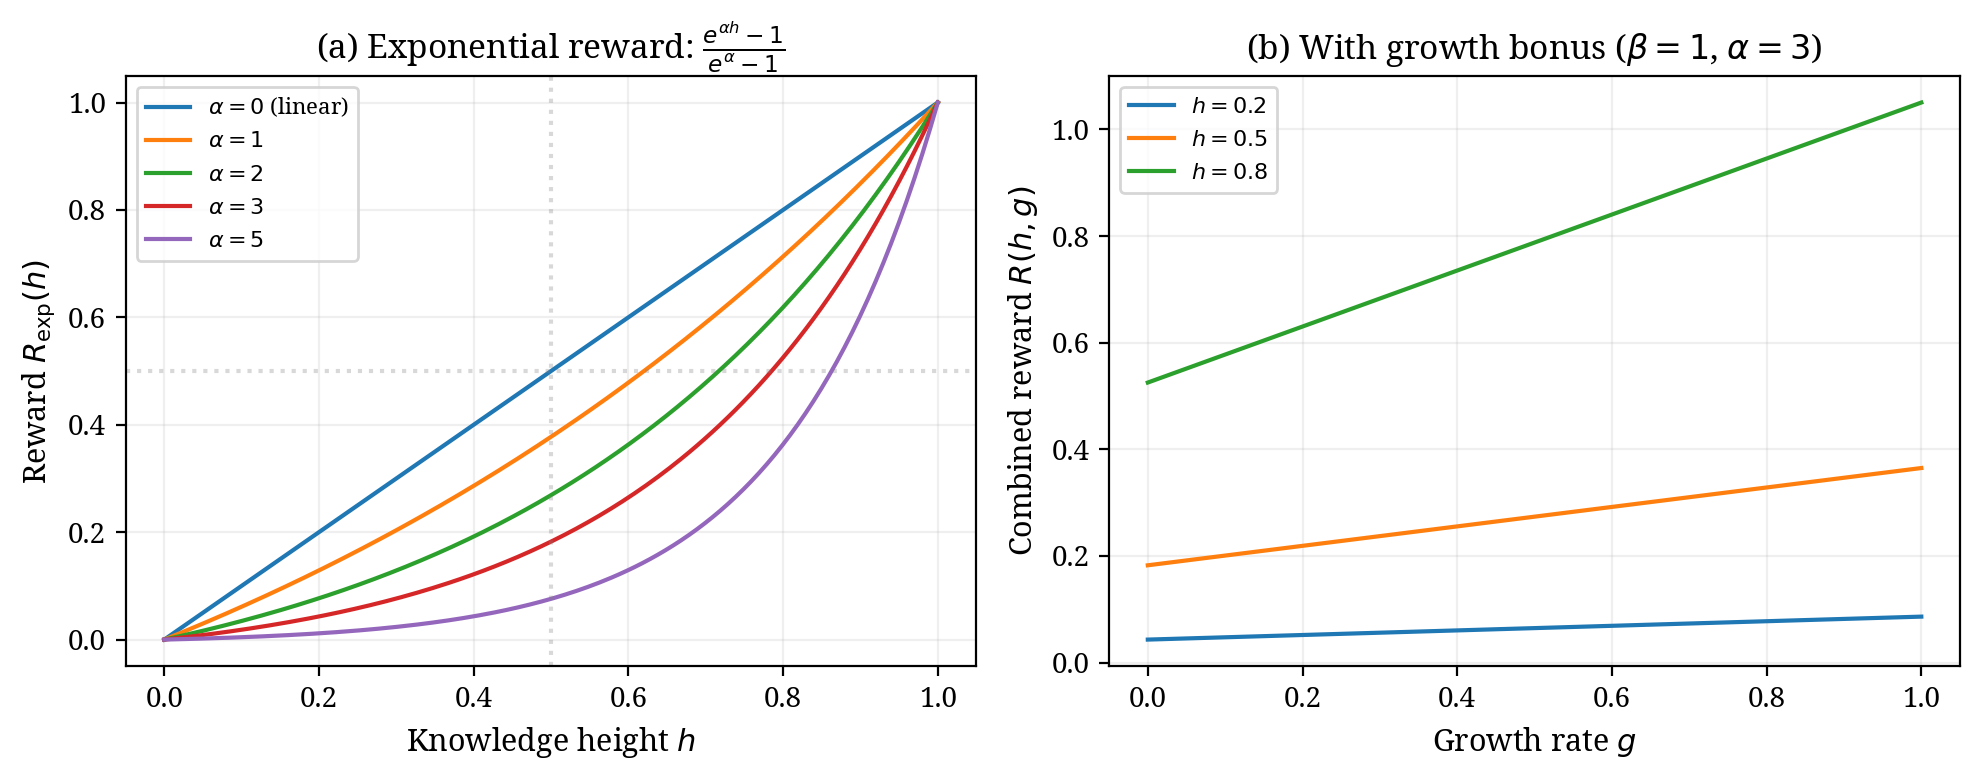
\includegraphics[width=\textwidth]{figures/fig3_reward_scaling.png}
\caption{Reward scaling functions. (a) The exponential position term creates winner-take-all dynamics, where teams at $h=0.8$ are substantially more rewarded than teams at $h=0.4$. (b) The combined reward includes a bonus for active knowledge growth.}
\end{figure}

\subsection{Reward-Modulated Social Learning}

In the base model, social learning shifts a particle's preferences toward its neighbors:
\begin{equation}
\mathbf{p}_i \leftarrow (1 - \eta_{\text{soc}})\mathbf{p}_i + \eta_{\text{soc}} \bar{\mathbf{p}}_{\mathcal{N}(i)}
\end{equation}
where $\bar{\mathbf{p}}_{\mathcal{N}(i)}$ is the unweighted mean of the neighbor preferences.

The Knowledge Manifold extension introduces a \textbf{reward-modulated social nudge}. Particles maintain an exponential moving average of their reward, $\bar{R}_i$. After the standard social learning step, an additional pass pulls particles toward their most successful neighbors, using weights proportional to neighbor reward:

\begin{equation}
w_{ij} = 1 + \rho \max(\bar{R}_j, 0)
\end{equation}
\begin{equation}
\mathbf{p}_i \leftarrow (1 - \eta_{\text{reward}}) \mathbf{p}_i + \eta_{\text{reward}} \sum_{j \in \mathcal{N}(i)} \frac{w_{ij}}{\sum_k w_{ik}} \mathbf{p}_j
\end{equation}

where $\rho$ is the social reward scale, and $\eta_{\text{reward}}$ is typically a fraction of $\eta_{\text{soc}}$ to avoid completely overriding the base dynamics. This creates a powerful macroeconomic effect: talent and attention naturally flow toward the most productive teams, driving further discovery in those regions.

\section{Simulation Results}

A typical 5-minute experiment (18,000 steps) demonstrates the interplay of these dynamics. 

\begin{figure}[H]
\centering
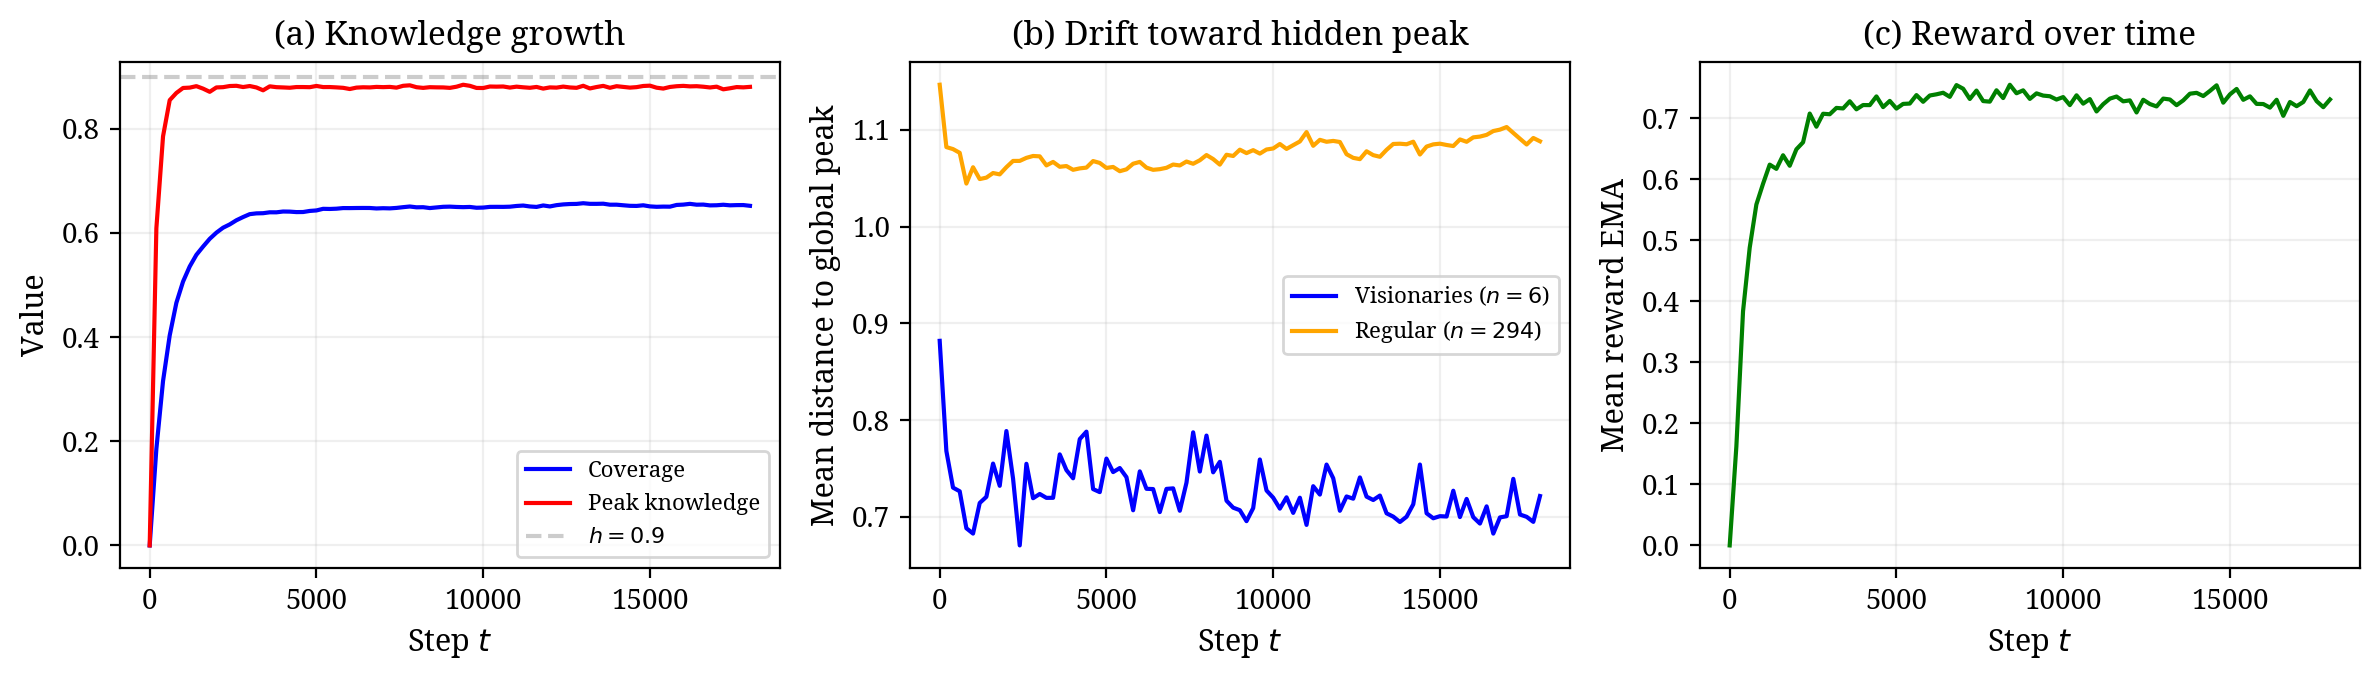
\includegraphics[width=\textwidth]{figures/fig5_dynamics.png}
\caption{(a) The peak knowledge quickly hits the structural ceiling, while overall coverage grows steadily. (b) Visionary particles (blue) drift significantly closer to the global hidden peak than regular particles (orange), demonstrating their role in guiding the organization. (c) Mean reward stabilizes as the organization optimizes its position.}
\end{figure}

\begin{figure}[H]
\centering
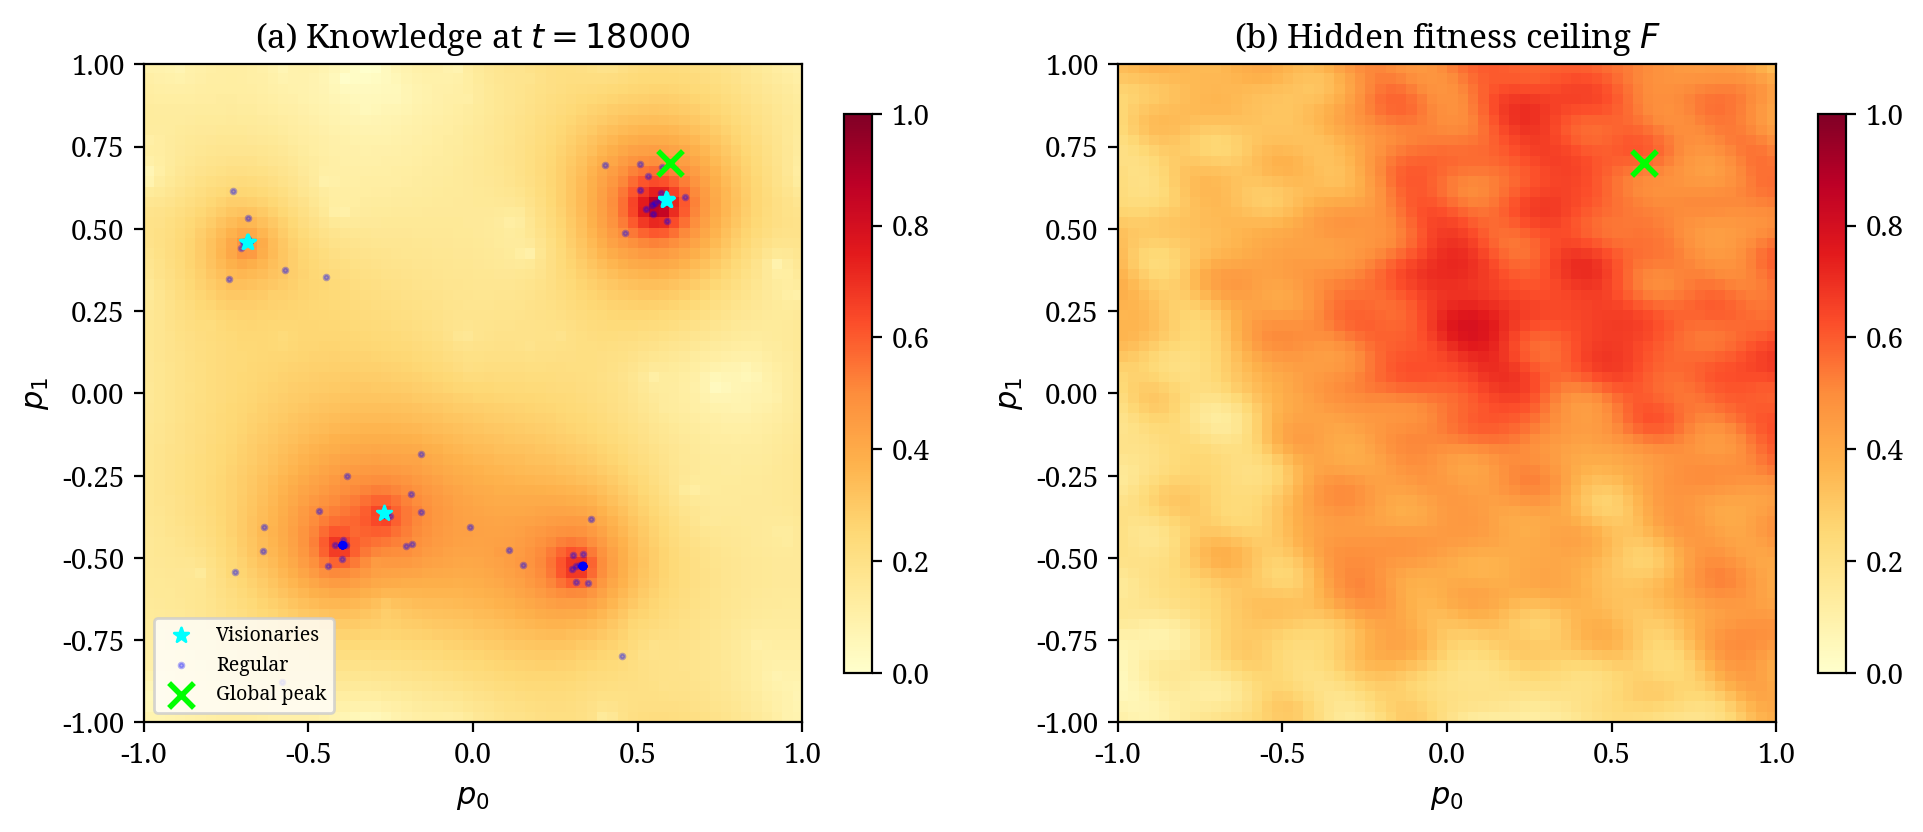
\includegraphics[width=\textwidth]{figures/fig6_final_state.png}
\caption{Comparison of the final knowledge manifold (a) and the hidden fitness ceiling (b). The organization has successfully discovered the major peaks, led by visionary particles (cyan stars) that tend to cluster near the global summit.}
\end{figure}

\end{document}
